\chapter{Anhang von Bildern}
\label{cha:anhang_bilder}
\begin{figure}[h!tb]
\centering
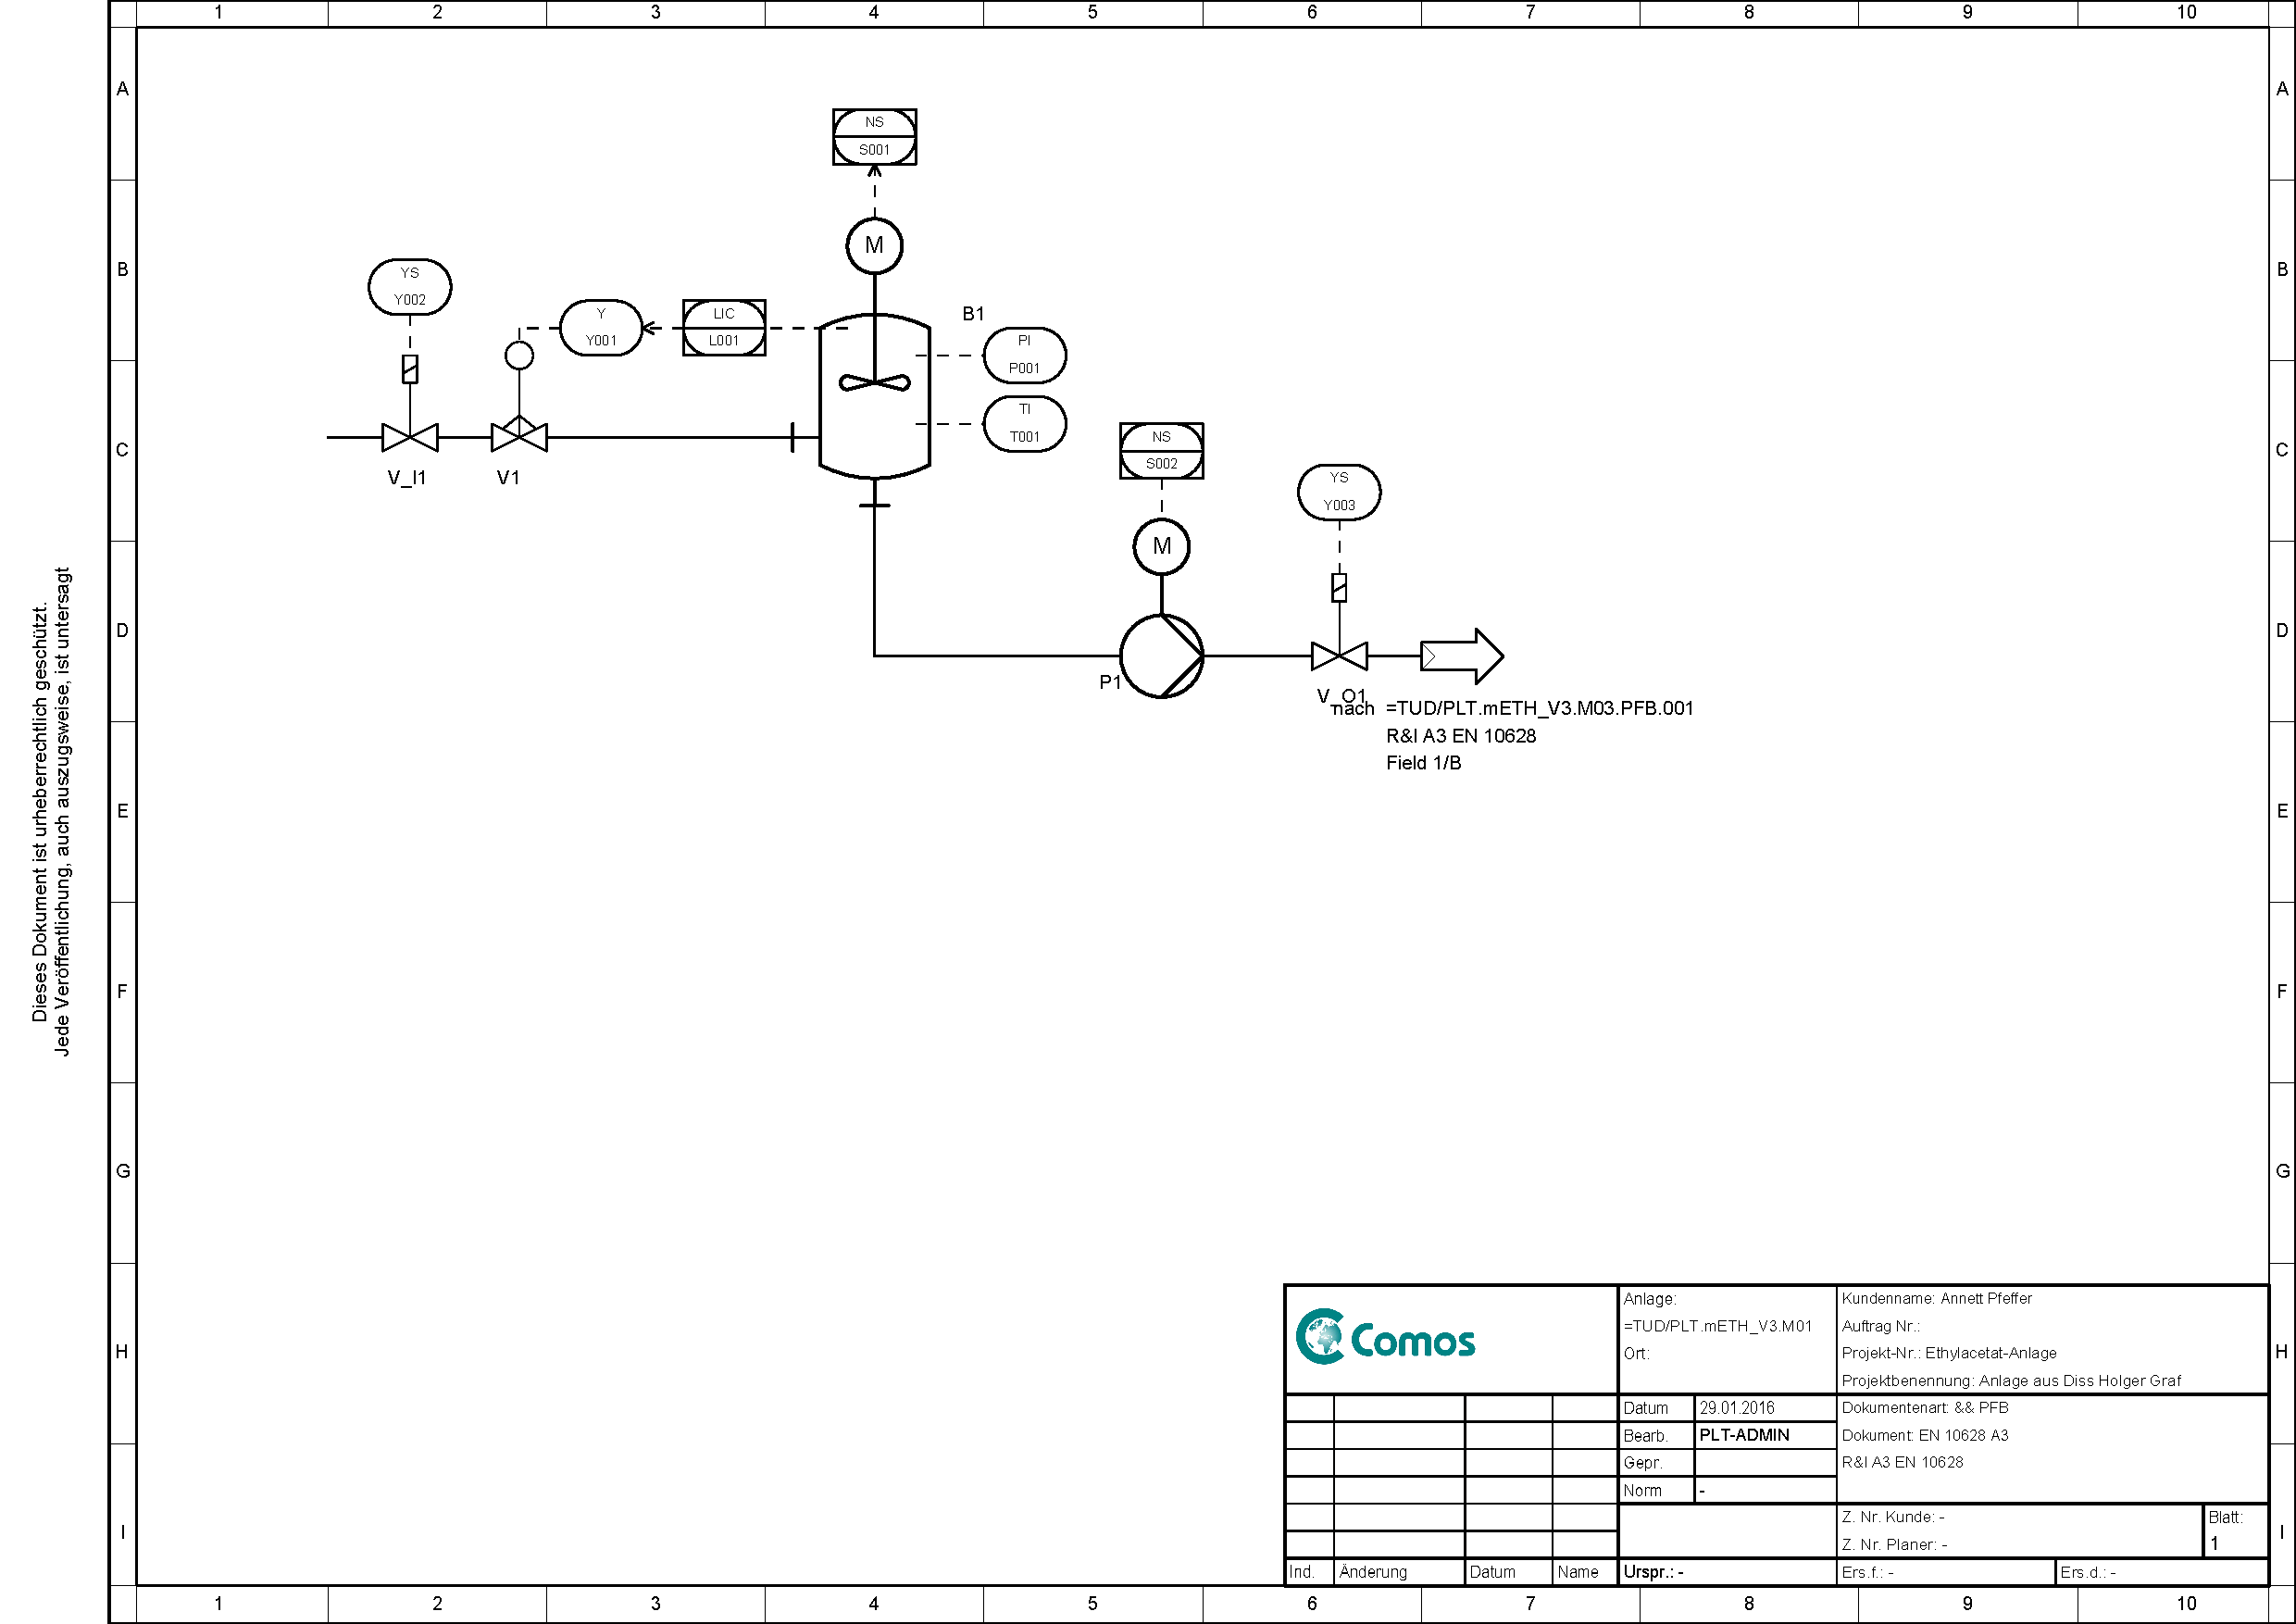
\includegraphics[height=\textwidth,angle=90]{bilder/M01_Vorlage_1_mit_Pumpe.pdf}
\caption[PID Modul 1]{Vorlagemodul 1 nach \cite{Pfeffer_2016}}
\label{fig:PIDMod1}
\end{figure}

\begin{figure}[h!tb]
\centering
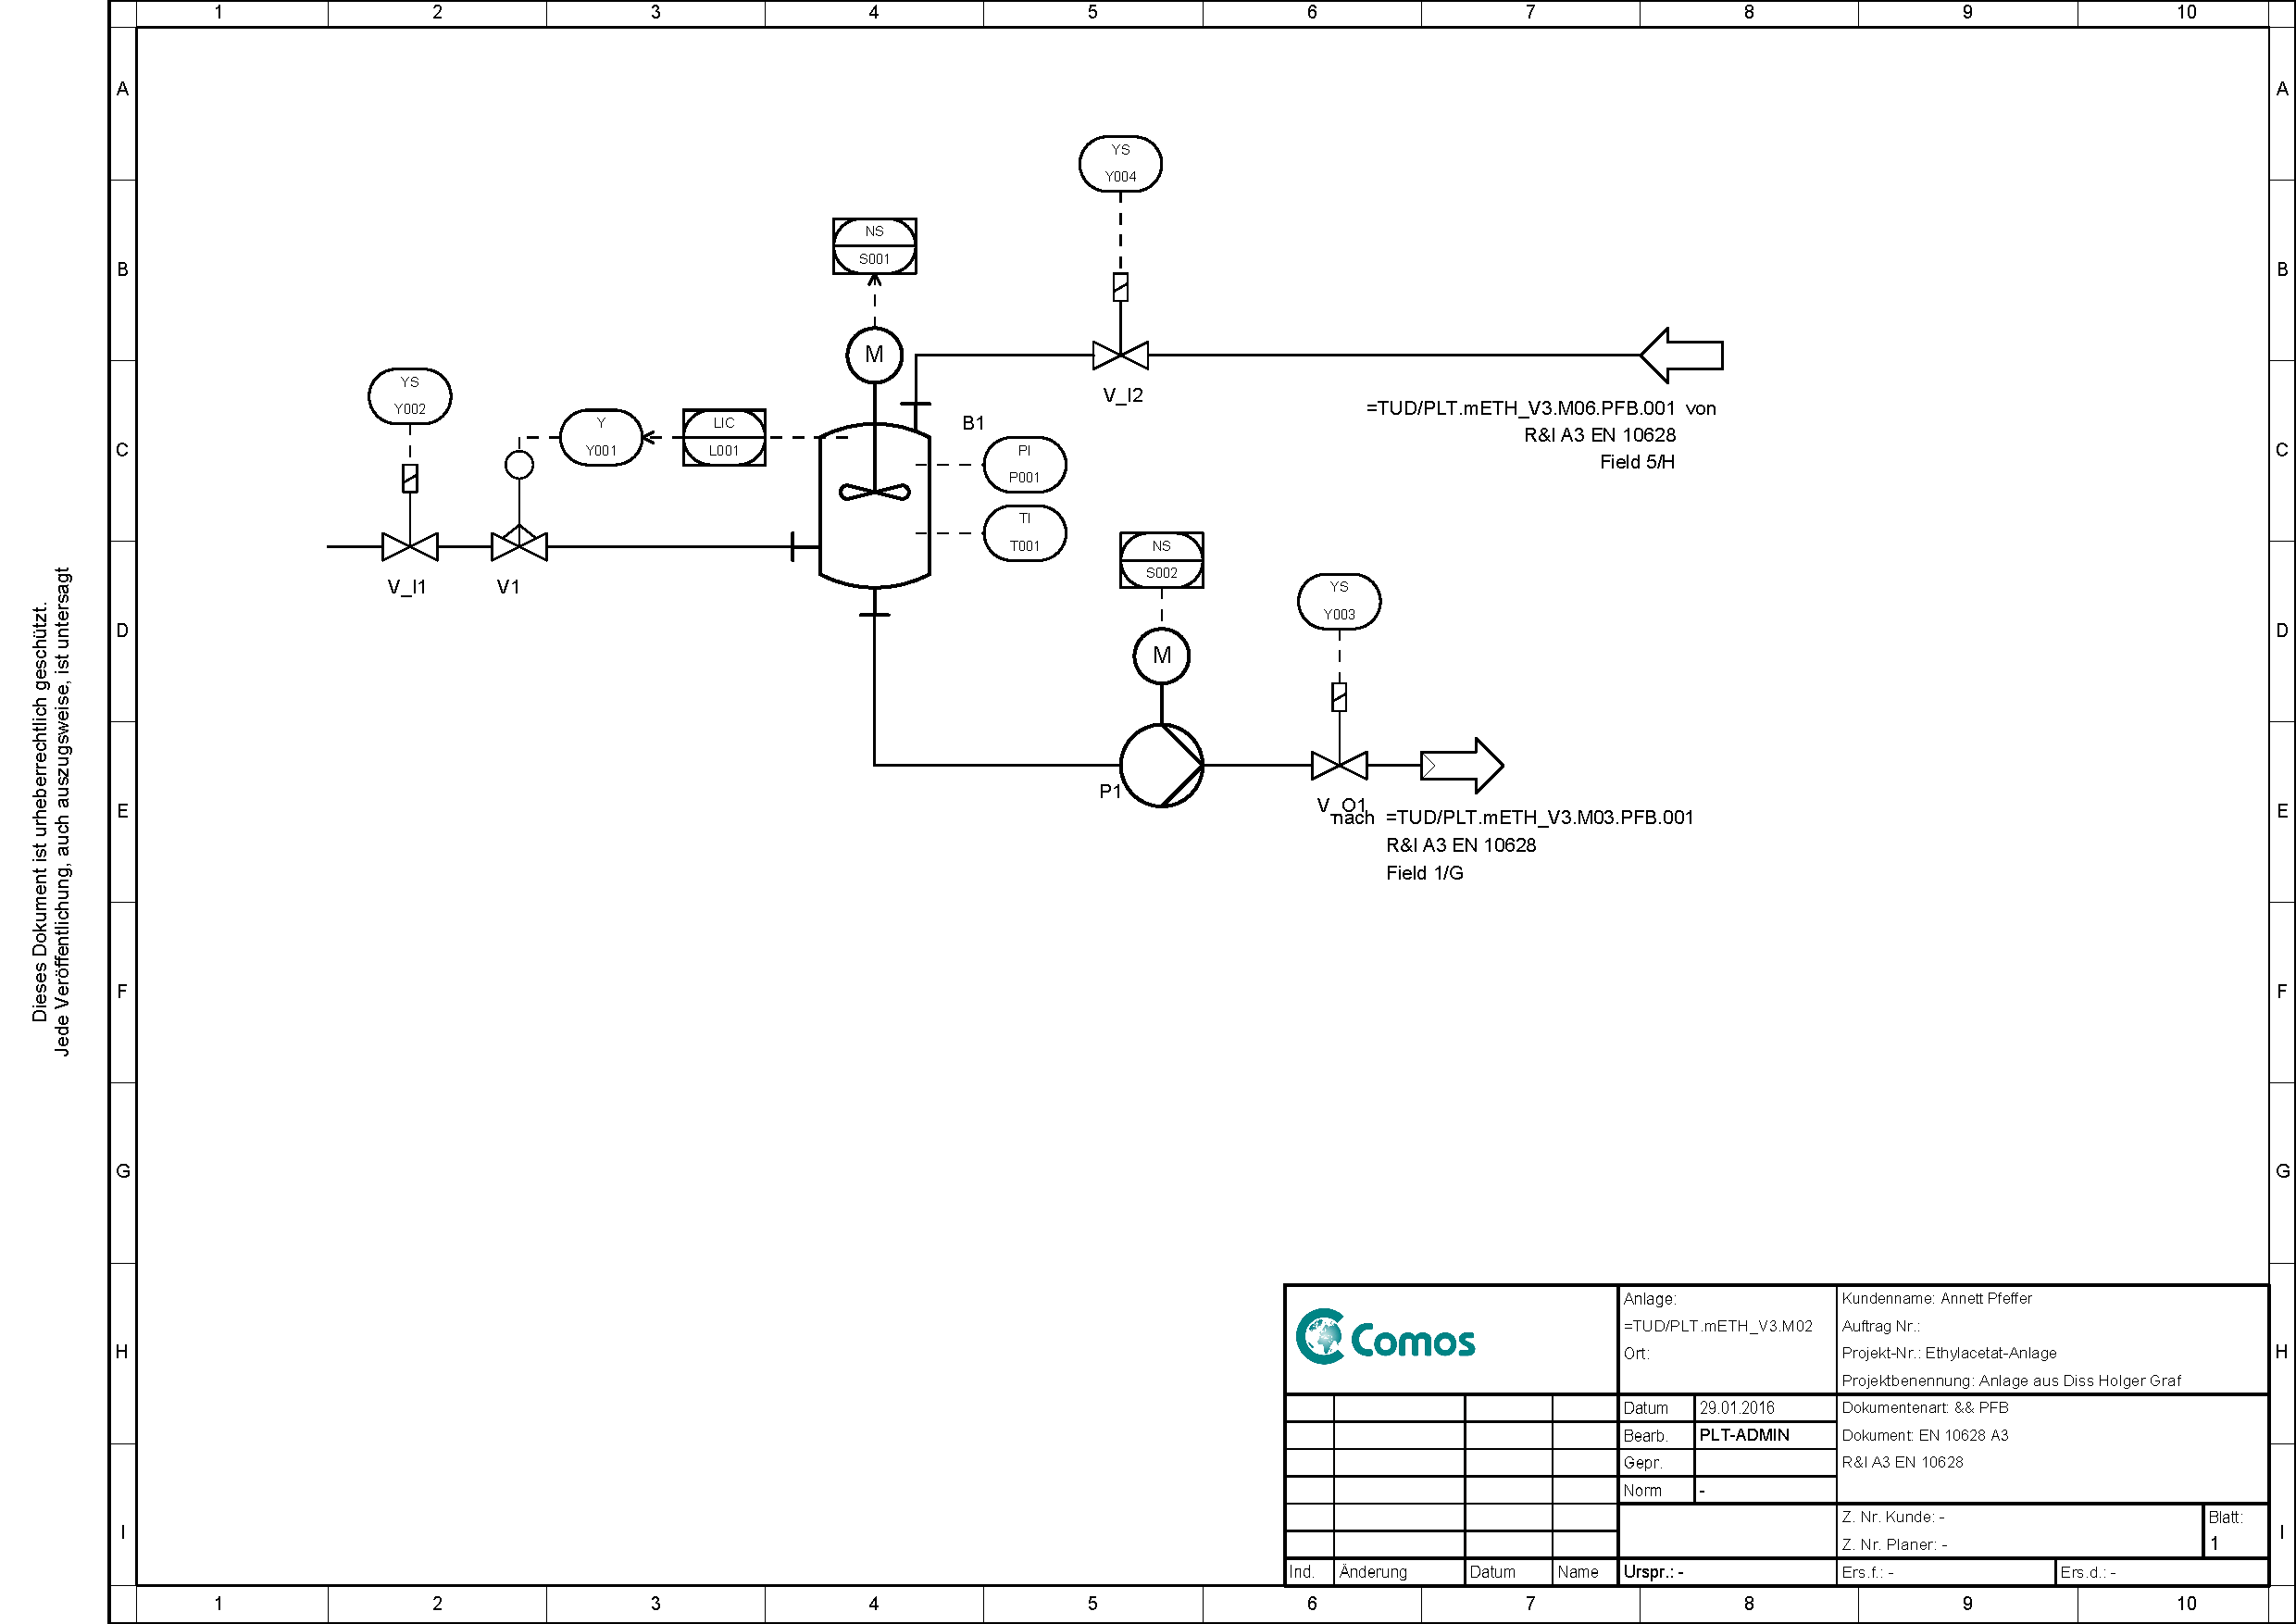
\includegraphics[height=\textwidth,angle=90]{bilder/M02_Vorlage_2_mit_Pumpe.pdf}
\caption[PID Modul 2]{Vorlagemodul 2 nach \cite{Pfeffer_2016}}
\label{fig:PIDMod2}
\end{figure}

\begin{figure}[h!tb]
\centering
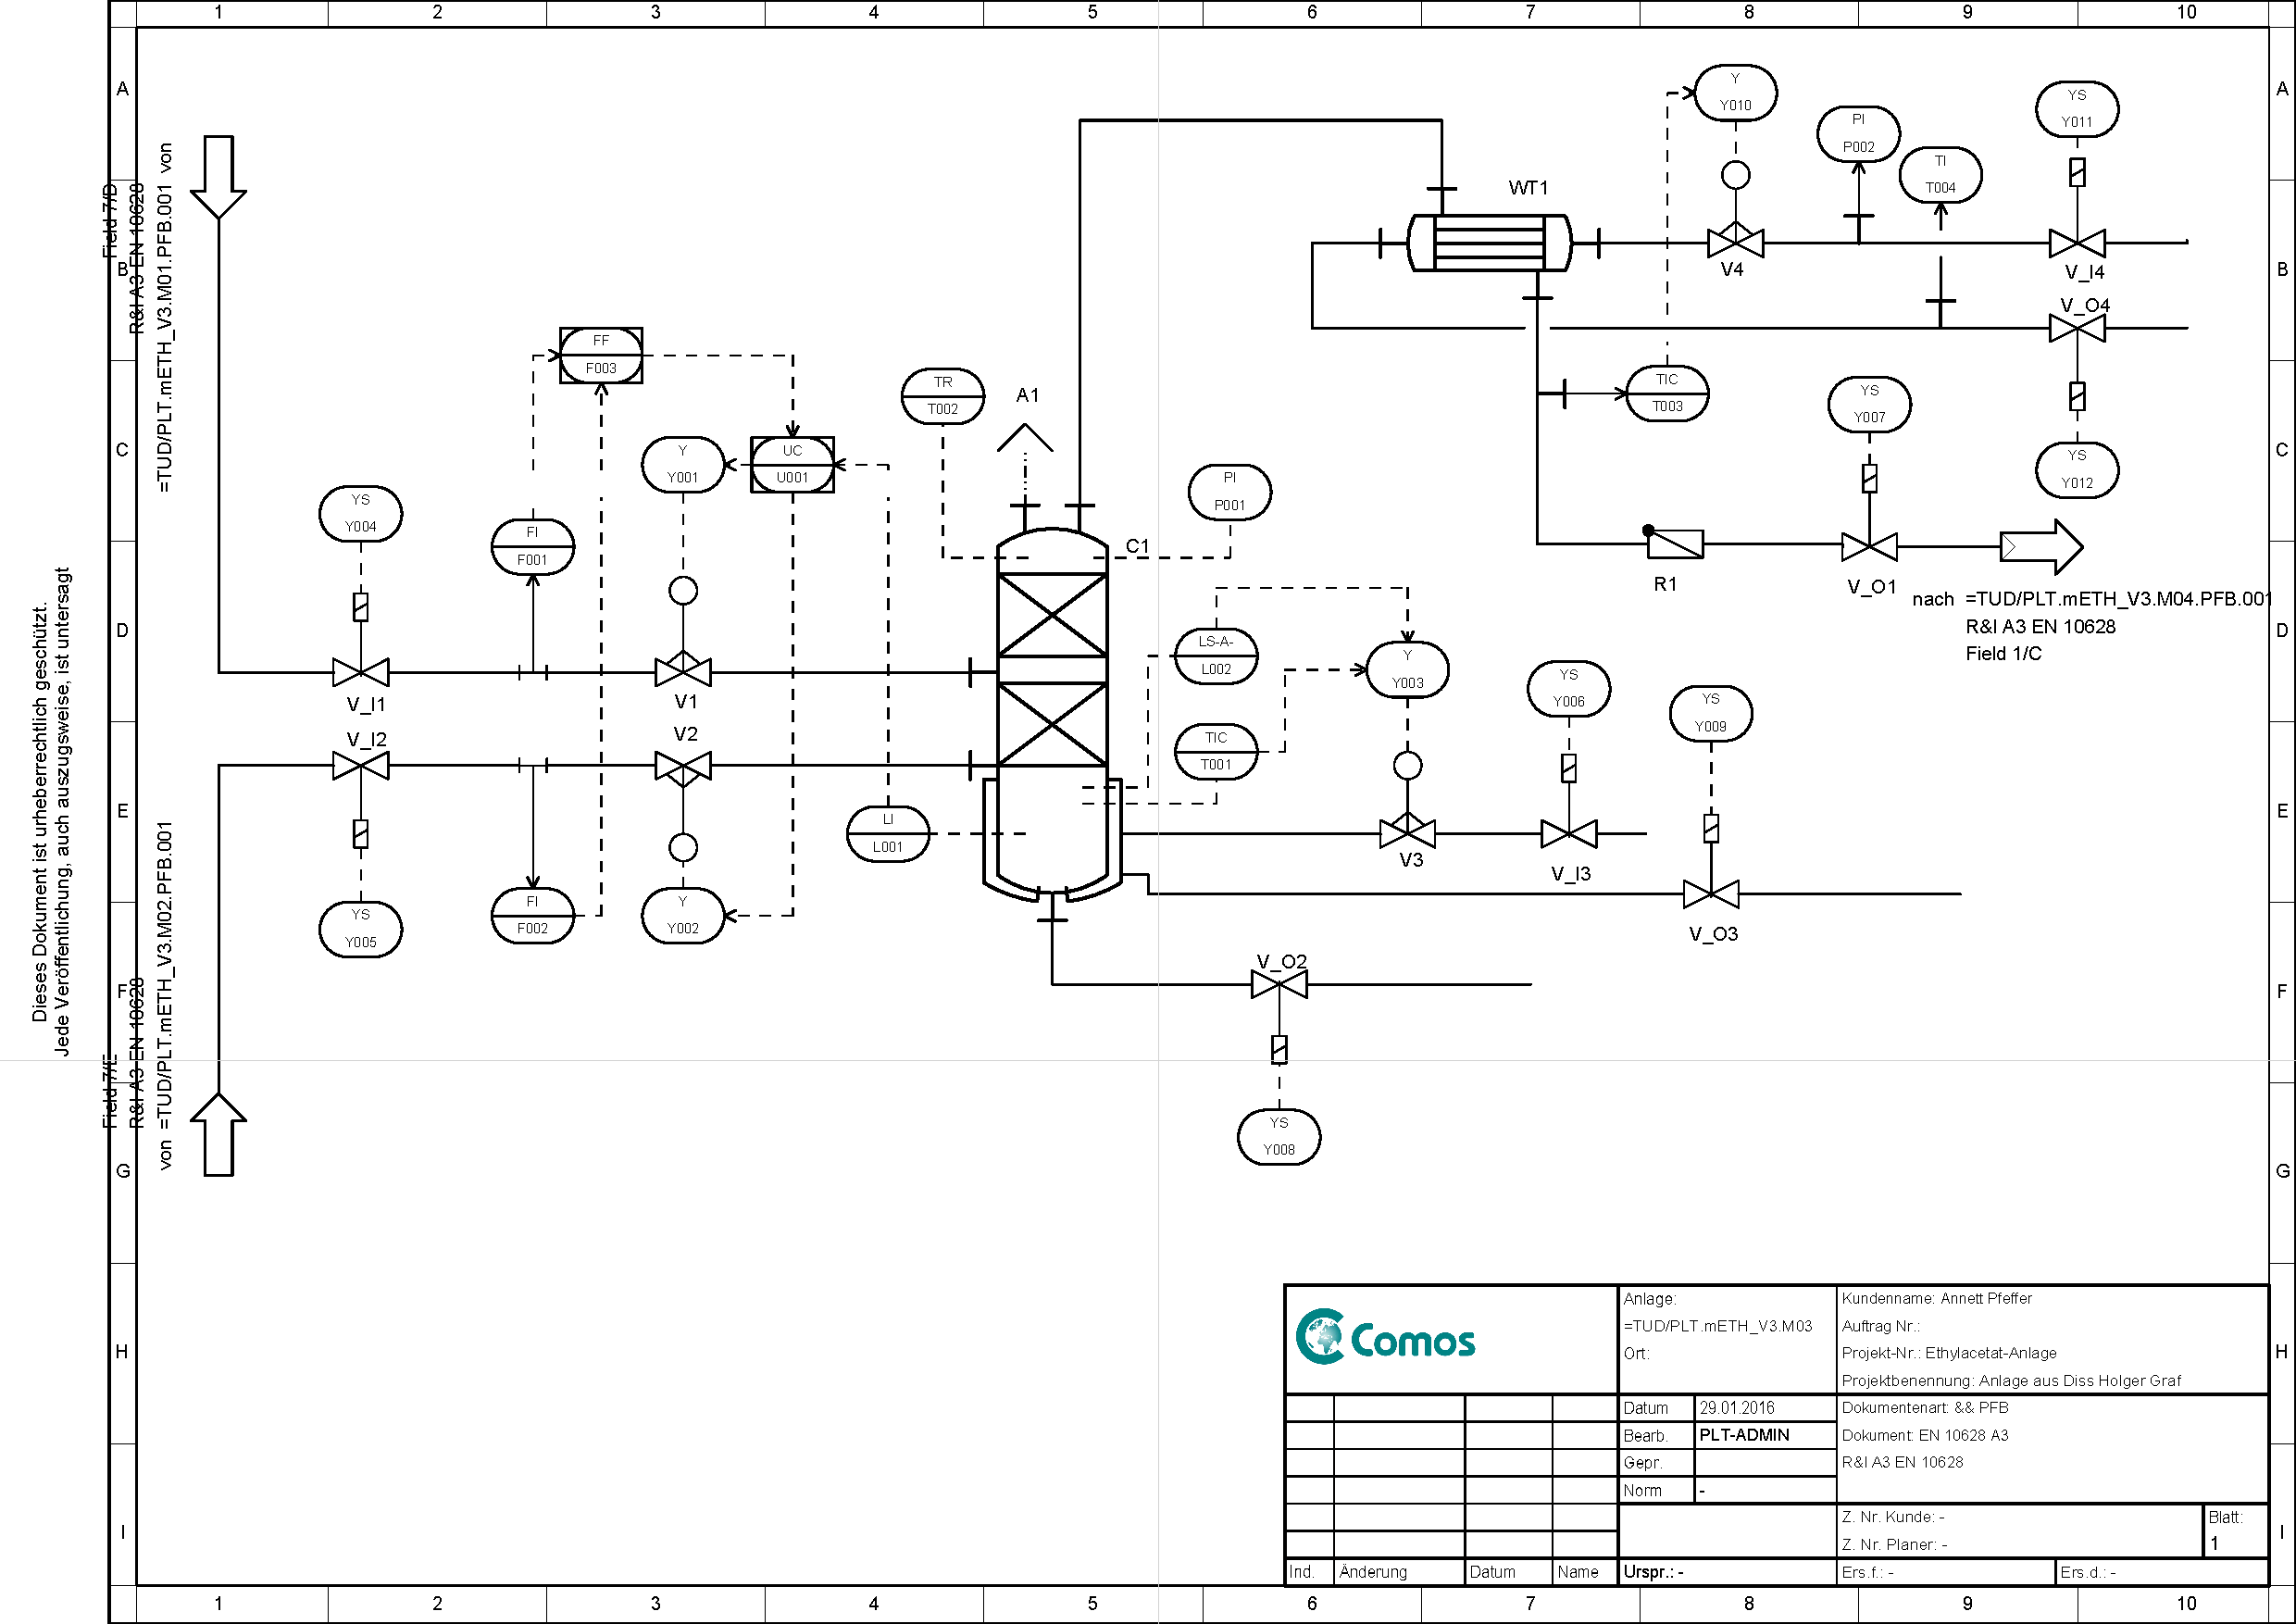
\includegraphics[height=\textwidth,angle=90]{bilder/M03_Kolonne_mit_Waermetauscher.pdf}
\caption[PID Modul 3]{Kolonne mit W\"armetauscher als Modul 3 nach \cite{Pfeffer_2016}}
\label{fig:PIDMod3}
\end{figure}

\chapter{Anhang von Tabellen} \label{cha:anhang_tabellen}
\begin{sidewaystable}[htb]
\tablestyle
\caption[HAZOP von Modul 1]{Ergebnisse der \ac{hazop} f\"ur das Tankmodul bezogen auf Durchfluss und F\"ullstand nach \cite{Pfeffer_2017}}
\begin{tabularx}{\textheight}{ccccCCCC}
\tableheadcolor
   {\tablehead ID} &
   {\tablehead unit} &
   {\tablehead Guide word} &
   {\tablehead Physical property} &
   {\tablehead consequences}&
   {\tablehead causes}&
   {\tablehead mechanisms for identification of deviation}&
   {\tablehead recommendation}
   \tabularnewline
%
\tablebody
  1 & in1 & no & flow & less level & valve(s) faulty OR control faulty OR externalcauses & - & - \\
  \hline 
  2 & in1 & more & flow & more level & valve faulty OR control faulty OR externalcauses & - & -  \\ 
  \hline 
  3 & in1 & less & flow & less level & valve(s) faulty OR control faulty OR externalcauses & - & - \\ 
  \hline 
  4 & tank & more & level & more pressure & ID=2 OR level sensor faulty & measure level & - \\ 
  \hline 
  5 & tank & no/less & level & no reactant $\mapsto$ damage pump & ID=1 OR ID=3 OR level sensor faulty OR leakage & measure level & - \\
  \hline  
  6 & out1 & no/less & flow & damage pump OR external consequences & pump faulty OR valve faulty OR ID=5 & - & - \\ 
  \hline 
  7 & out1 & more & flow & damage pump OR external consequences & pump faulty OR ID=4 OR ID=6 & - & - \\ 
  \hline 
  8 & out1 & reverse & flow & pollution of reactant & pump faulty OR external causes & - & - 
   \tabularnewline
%
\tableend
\end{tabularx}
\label{tab:hazopBsp_M1}
\end{sidewaystable}

\begin{sidewaystable}[htb]
\tablestyle
\caption[HAZOP von Modul 3]{Ergebnisse der \ac{hazop} f\"ur das Modul 3 bestehend aus Kolonne und W\"armetauscher bezogen auf Durchfluss und F\"ullstand nach \cite{Pfeffer_2017}}
\begin{tabularx}{\textheight}{ccccCCCc}
\tableheadcolor
   {\tablehead ID} &
   {\tablehead unit} &
   {\tablehead Guide word} &
   {\tablehead Physical property} &
   {\tablehead consequences}&
   {\tablehead causes}&
   {\tablehead mechanisms for identification of deviation}&
   {\tablehead recommendation}
   \tabularnewline
1	&	in1	&	no	&	flow	&	unknown (no reaction?)	&	valve(s) faulty OR flow/level control faulty OR external causes	&	measure flow	&	-	\\ \hline
2	&	in1	&	more	&	flow	&	changed reaction balance	&	valve(s) faulty OR flow/level control faulty OR external causes	&	measure flow	&	-	\\ \hline
3	&	in1	&	less	&	flow	&	changed reaction balance	&	valve(s) faulty OR flow/level control faulty OR external causes	&	measure flow	&	-	\\ \hline
4	&	in2	&	no	&	flow	&	no reaction	&	valve(s) faulty OR flow/level control faulty OR external causes	&	measure flow	&	-	\\ \hline
5	&	in2	&	more	&	flow	&	changed reaction balance	&	valve(s) faulty OR flow/level control faulty OR external causes	&	measure flow	&	-	\\ \hline
6	&	in2	&	less	&	flow	&	changed reaction balance	&	valve(s) faulty OR flow/level control faulty OR external causes	&	measure flow	&	-	\\ \hline
7	&	coloumn	&	more	&	level	&	changed reaction balance	&	ID=2 OR ID=5	&	measure level	&	-	\\ \hline
8	&	coloumn	&	less	&	level	&	changed reaction balance	&	ID=1 OR ID=3 OR ID=4 OR ID=6 OR leakage 	&	measure level	&	-	
\tablebody
   \tabularnewline
%
\tableend
\end{tabularx}
\label{tab:hazopBsp_M3}
\end{sidewaystable}


%%\begin{table}[h!tb] %if possible put table here else at top or bottom of page
%%\centering %Tabelle wird auf der Seite zentriert
%%%\begin{tabularx}{<width}>{<preambel>}
%%\begin{tabularx}{\linewidth}{@{\extracolsep{\fill}}X|X|X|X|X|X|X@{\extracolsep{\fill}}} %make table as wide as text
%%\toprule %Tabellenanfang
%%% Kopfzeile
%%ID & unit & deviation & causes & consequences & mechanisms for
%%identification of deviation & recommendations \\
%%\midrule %Trennung von Kopf und Inhalt
%%% Inhalt
%%1 & in 1 & less flow & valve(s) faulty (closed, less open, clogged) & less level & - & - \\
%%\bottomrule %Tabellenschluss
%%\end{tabularx}
%%\caption{Ergebnisse einer \ac{hazop} f\"ur einen Tank}
%%\label{tab:hazopBsp} %reference with \prettyref{tab:•}
%%\end{table} 
%\begin{sidewaystable}[htb]
%\tablestyle
%\caption{Ergebnisse einer \ac{hazop} f\"ur einen Tank}
%%\begin{tabularx}{\textwidth}{*{10}{>{\centering\arraybackslash}X}}%
%%\begin{tabularx}{\textheight}{M{0.25cm}M{0.35cm}YM{2.1cm}YM{4.1cm}M{5.1cm}Y}
%\begin{tabularx}{\textheight}{ccccCCCC}
%\tableheadcolor
%%   \multicolumn{1}{c}{\tablehead ID} &
%%   \multicolumn{1}{c}{\tablehead unit} &
%%   \multicolumn{1}{c}{\tablehead Guide word} &
%%   \multicolumn{1}{c}{\tablehead \parbox{2.0cm}{Physical \newline property}} &
%%   \multicolumn{1}{c}{\tablehead consequences}&
%%   \multicolumn{1}{c}{\tablehead \parbox{4.0cm}{causes}}&
%%   \multicolumn{1}{c}{\tablehead \parbox{5cm}{mechanisms for \newline identification of deviation}}&
%%   \multicolumn{1}{c}{\tablehead recommendation}
%%   \tabularnewline
%%    \multirow{2}{*}{\tablehead ID} &
%%    \multirow{2}{*}{\tablehead unit} &
%%    {\tablehead Guide} &
%%    {\tablehead Physical} &
%%    \multirow{2}{*}{\tablehead consequences} &
%%    \multirow{2}{*}{\tablehead causes} &
%%    {\tablehead mechanisms for}&
%%    \multicolumn{1}{c}{\tablehead recommendation} \\
%%
%%    &
%%    &
%%    {\tablehead word}&
%%    {\tablehead property}&
%%    &
%%    &
%%    {\tablehead identification of deviation} &  
%   {\tablehead ID} &
%   {\tablehead unit} &
%   {\tablehead Guide word} &
%   {\tablehead Physical property} &
%   {\tablehead consequences}&
%   {\tablehead causes}&
%   {\tablehead mechanisms for identification of deviation}&
%   {\tablehead recommendation}
%   \tabularnewline
%%
%\tablebody
%  1 & in1 & no & flow & less level & valve(s) faulty OR control faulty OR externalcauses & - & - \\
%  \hline 
%  2 & in1 & more & flow & more level & valve faulty OR control faulty OR externalcauses & - & -  \\ 
%  \hline 
%  3 & in1 & less & flow & less level & valve(s) faulty OR control faulty OR externalcauses & - & - \\ 
%  \hline 
%  4 & tank & more & level & more pressure & ID=2 OR level sensor faulty & measure level & - \\ 
%  \hline 
%  5 & tank & no/less & level & no reactant $\mapsto$ damage pump & ID=1 OR ID=3 OR level sensor faulty OR leakage & measure level & - \\
%  \hline  
%  6 & out1 & no/less & flow & damage pump OR external consequences & pump faulty OR valve faulty OR ID=5 & - & - \\ 
%  \hline 
%  7 & out1 & more & flow & damage pump OR external consequences & pump faulty OR ID=4 OR ID=6 & - & - \\ 
%  \hline 
%  8 & out1 & reverse & flow & pollution of reactant & pump faulty OR external causes & - & - 
%   \tabularnewline
%%
%\tableend
%\end{tabularx}
%\label{tab:hazopBsp}
%\end{sidewaystable}